\documentclass[tikz,border=6pt]{standalone}
\usepackage{xcolor}
\usetikzlibrary{calc}

\definecolor{mainblue}{HTML}{001158}
\definecolor{accent}{HTML}{8592bc}
\definecolor{lightaccent}{HTML}{e7e9f2}

\begin{document}
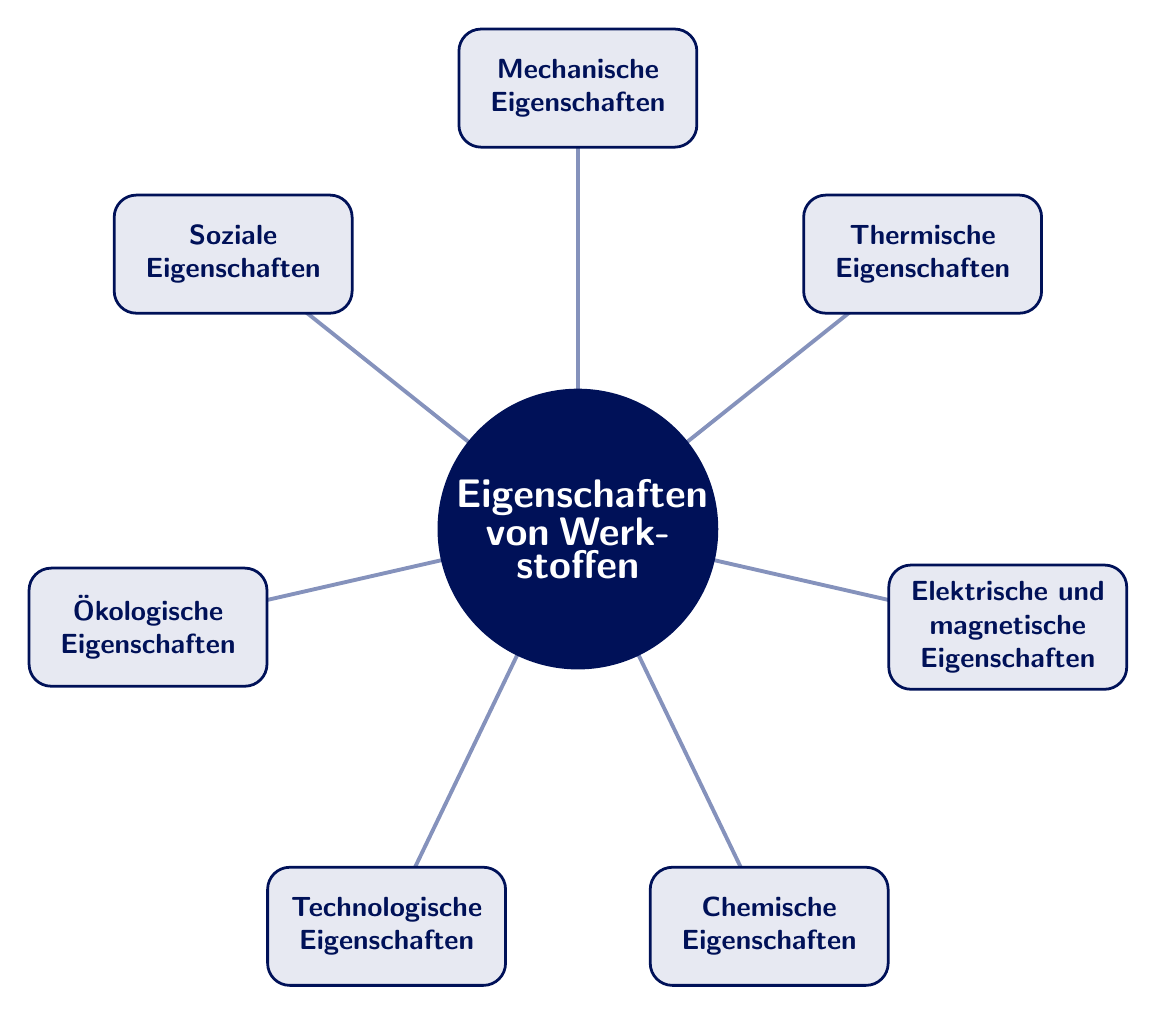
\begin{tikzpicture}[
    font=\sffamily,
    center/.style={
        circle, draw=mainblue, fill=mainblue, text=white,
        align=center, text width=3.1cm, inner sep=2pt, line width=1pt
    },
    petal/.style={
        rectangle, rounded corners=8pt, draw=mainblue, fill=lightaccent, text=mainblue,
        align=center, text width=2.6cm, minimum height=1.5cm,
        line width=1pt, font=\sffamily\bfseries, inner sep=6pt
    },
    spoke/.style={draw=accent, line width=1.4pt}
]

\def\R{5.6cm}

\foreach \i/\lbl in {
    0/Mechanische Eigenschaften,
    1/Thermische Eigenschaften,
    2/Elektrische und magnetische Eigenschaften,
    3/Chemische Eigenschaften,
    4/Technologische Eigenschaften,
    5/Ökologische Eigenschaften,
    6/Soziale Eigenschaften
} {
    \pgfmathsetmacro{\angle}{90 - \i*360/7}
    \draw[spoke] (0,0) -- (\angle:\R);
}

\node[center] (center) at (0,0) {\Large\bfseries Eigenschaften von Werkstoffen};

\foreach \i/\lbl in {
    0/Mechanische Eigenschaften,
    1/Thermische Eigenschaften,
    2/Elektrische und magnetische Eigenschaften,
    3/Chemische Eigenschaften,
    4/Technologische Eigenschaften,
    5/Ökologische Eigenschaften,
    6/Soziale Eigenschaften
} {
    \pgfmathsetmacro{\angle}{90 - \i*360/7}
    \node[petal] (N\i) at (\angle:\R) {\lbl};
}

\end{tikzpicture}
\end{document}
